\documentclass[
  captions=tableheading,
  bibliography=totoc, 
  titepage=firstiscover,
]{scrartcl}

\usepackage{blindtext} %neuer input

\usepackage{longtable} % Tabellen über mehrere Seiten

\usepackage[utf8]{inputenc} %neuer input

\usepackage{scrhack}

\usepackage[aux]{rerunfilecheck} %Warnung falls nochmal kompiliert werden muss

\usepackage{fontspec} %Fonteinstellungen

\recalctypearea{}

\usepackage[main=ngerman]{babel} %deutsche Spracheinstellung

\usepackage{ragged2e} %neuer input

\usepackage{amsmath, nccmath}

\usepackage{amssymb} %viele mathe Symbole

\usepackage{mathtools} %Erweiterungen für amsmath


\DeclarePairedDelimiter{\abs}{\lvert}{\rvert}
\DeclarePairedDelimiter{\norm}{\lVert}{\rVert}

\DeclarePairedDelimiter{\bra}{\langle}{\rvert}
\DeclarePairedDelimiter{\ket}{\lvert}{\rangle}

\DeclarePairedDelimiterX{\braket}[2]{\langle}{\rangle}{
#1 \delimsize| #2
}

\NewDocumentCommand \dif {m}
{
\mathinner{\symup{d} #1}
}


\usepackage[
  math-style=ISO,
  bold-style=ISO,
  sans-style=italic,
  nabla=upright,
  partial=upright,
  warnings-off={
    mathtools-colon,
    mathtools-overbracket,
  },
]{unicode-math}

\setmathfont{Latin Modern Math}
\setmathfont{XITS Math}[range={scr, bfscr}]
\setmathfont{XITS Math}[range={cal, bfcal}, StylisticSet=1]


\usepackage[
  locale=DE,
  separate-uncertainty=true,
  per-mode=reciprocal,
  output-decimal-marker={,},
]{siunitx}

\usepackage[autostyle]{csquotes} %richtige Anführungszeichen

\usepackage{xfrac}

\usepackage{float}

\floatplacement{figure}{htbp}

\floatplacement{table}{htbp}

\usepackage[ %floats innerhalb einer section halten
  section,   %floats innerhalb er section halten
  below,     %unterhalb der Section aber auf der selben Seite ist ok
]{placeins}

\usepackage[
  labelfont=bf,
  font=small,
  width=0.9\textwidth,
]{caption}

\usepackage{subcaption} %subfigure, subtable, subref

\usepackage{graphicx}

\usepackage{grffile}

\usepackage{booktabs}

\usepackage{microtype} %Verbesserungen am Schriftbild

\usepackage[
backend=biber,
]{biblatex}

\addbibresource{../lit.bib}

\usepackage[ %Hyperlinks im Dokument
  german,
  unicode,
  pdfusetitle,
  pdfcreator={},
  pdfproducer={},
]{hyperref}

\usepackage{bookmark}

\usepackage[shortcuts]{extdash}

%\usepackage{warpcol}


\begin{document}
    \title{ATP Übungsblatt 3}
    \author{  
    Tobias Rücker\\
    \texorpdfstring{\href{mailto:tobias.ruecker@tu-dortmund.de}{tobias.ruecker@tu-dortmund.de}
    \and}{,} 
    Paul Störbrock\\
    \texorpdfstring{\href{mailto:paul.stoerbrock@tu-dortmund.de}{paul.stoerbrock@tu-dortmund.de}}{}
    }
\maketitle
\center{\Large Abgabegruppe: \textbf{Mittw. 10-12 Uhr}}
\thispagestyle{empty}

\newpage
\tableofcontents
\thispagestyle{empty}
\newpage

\setcounter{page}{1}


\section{Aufgabe 7}

    \begin{figure}[H]
        \centering
        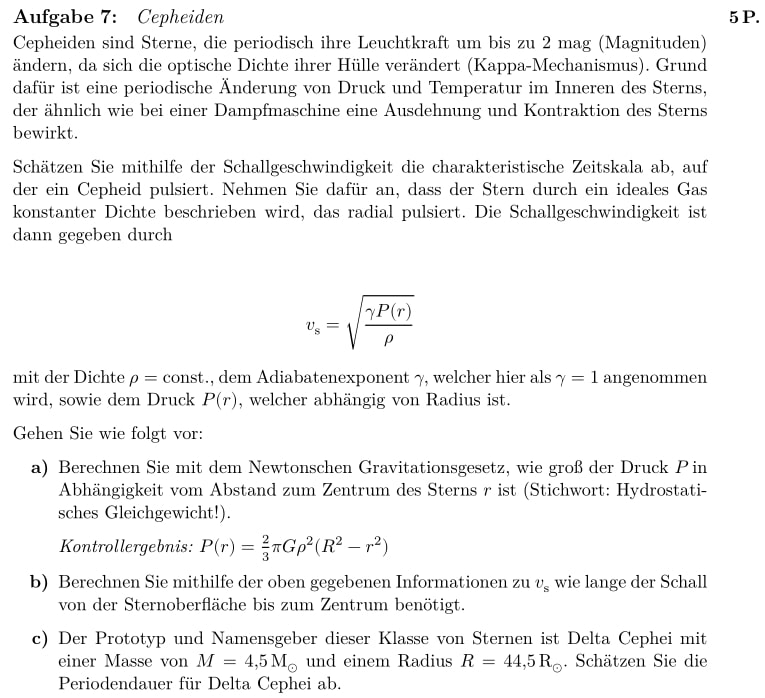
\includegraphics[width=\textwidth]{images/Aufgabe7abc.jpg}
        \label{fig:1}
    \end{figure}
    \begin{figure}[H]
        \centering
        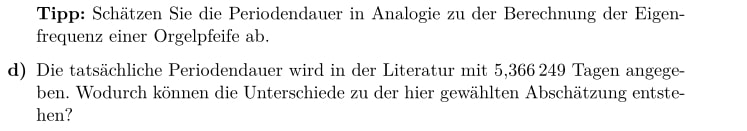
\includegraphics[width=\textwidth]{images/Aufgabe7d.jpg}
        \label{fig:2}
    \end{figure}

    \flushleft{\;}\justifying

\newpage
\subsection{a)}

Aus dem letzten Blatt:
\begin{align}
    \frac{GM \varrho}{r^2}= \frac{\symup{d}p}{\symup{d}r}\\
    \intertext{
        Nebenrechnung:
    }
    M = \varrho \cdot varrho\\
    = \varrho \frac{4}{3} \pi r^3\\
    \intertext{
        Ende Nebenrechnung
    }
    -\frac{4}{3}\pi G \varho ^2 r = \frac{dP}{dr} \vert \int_r^R \syup{d} r'\\
    -\frac{4}{3}\pi G \varho ^2 \int_r^R r' \symup{d} r' = \int_r^R \frac{dP}{dr'} \symup{d} r'\\
    -\frac{2}{3} \pi  G \varrho ^2 (R^2 -r^2) = \underbrace{P(R)}_{=0} -P(r)
    \intertext{
        Am Rand der Sonne wirkt keine Kraft wegen dem hydrostatischen Gleichgewicht, daher wirdder Druck an der Stelle 0.
    } 
    P(r)=\frac{2}{3} \pi  G \varrho ^2 (R^2 -r^2)
\end{align}


\subsection{b)}

\begin{align}
    v_s = \sqrt{\frac{\gamma P(r)}{\varrho} }\\
    v_s = \sqrt{\frac{2}{3} \pi \gamma \varrho G (R^2-r^2)}\\
    \gamma =1\\
    \frac{dr}{dt}= v_s\\
    dt = \frac{1}{v_s} dr \vert \int \\
    \int _0^t 1 dt = \int _0^R \sqrt{\frac{3}{2G \varrho \pi}} \frac{1}{(R^2-r^2)^{\frac{1}{2}}} dr \\
    t= \int _0^R \sqrt{\frac{3}{2G \varrho \pi}} \frac{1}{R\sqrt{1-\frac{r^2}{R^2}}} dr\\
    \intertext{
        Substitution
    }
    \frac{r}{R}=u\\
    \frac{du}{dr}=\frac{1}{R}\\
    dr = du R\\
    \intertext {
        Weiter
    }
    =\sqrt{\frac{3}{2G \varrho \pi}} \int_^1 \frac{1}{\sqrt{1-u^2}} du\\
    =\sqrt{\frac{3}{2G \varrho \pi}} \arcsin(U) \vert_0^1 \\
    =\sqrt{\frac{3}{2G \varrho \pi}} \frac{\pi}{2}
\end{align}



\subsection{c)}



\subsection{d)}



\section{Aufgabe 8}

\begin{figure}[H]
    \centering
    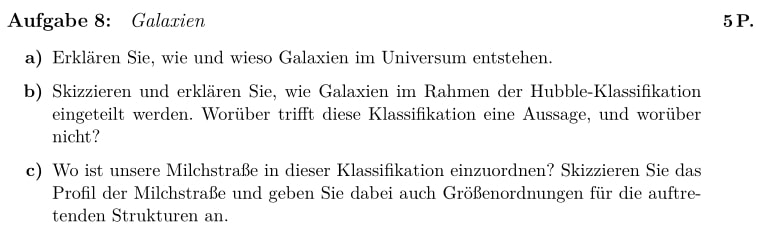
\includegraphics[width=\textwidth]{images/Aufgabe8.jpg}
    \label{fig:3}
\end{figure}

\newpage
\subsection{a)}



\subsection{b)}



\subsection{c)}



\section{Aufgabe 9}

\begin{figure}[H]
    \centering
    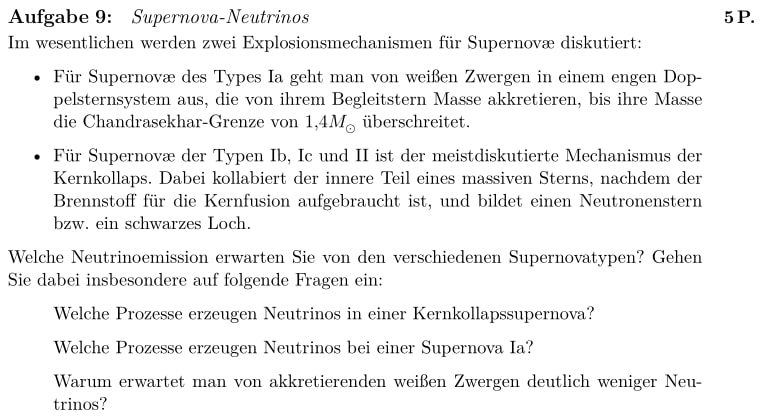
\includegraphics[width=\textwidth]{images/Aufgabe9.jpg}
    \label{fig:4}
\end{figure}



\end{document}
